\documentclass[12pt]{article}
\usepackage{graphicx}
\usepackage{wrapfig}
\usepackage{subfigure}
\usepackage{multirow}
\usepackage{hyperref}
\usepackage{amsmath}
\usepackage{amssymb}
%\usepackage{ngerman}
\usepackage[ansinew]{inputenc}
\usepackage[left=2cm,top=1cm]{geometry}

% vector graphics test
\usepackage{color}
\usepackage{transparent}
\graphicspath{{graphs/}}

\setlength{\parindent}{0pt}




\begin{document}
	\pagestyle{empty}
	\textasciitilde

\begin{titlepage}
	\centering
	\bigskip
	\huge{Astronomisches Praktikum: Altersbestimmung offener Sternhaufen}\\
	\bigskip
	\large{Versuch 4}\\
	\bigskip
	\large{Jan R\"{o}der \& Julia Lienert}
	\bigskip
	\tableofcontents
\end{titlepage}

\pagebreak


\section{Einleitung}

\section{Analyse eines unbekannten Sternhaufens}

\subsection{Aufgabe 1}

\begin{figure} [h]
	\centering
	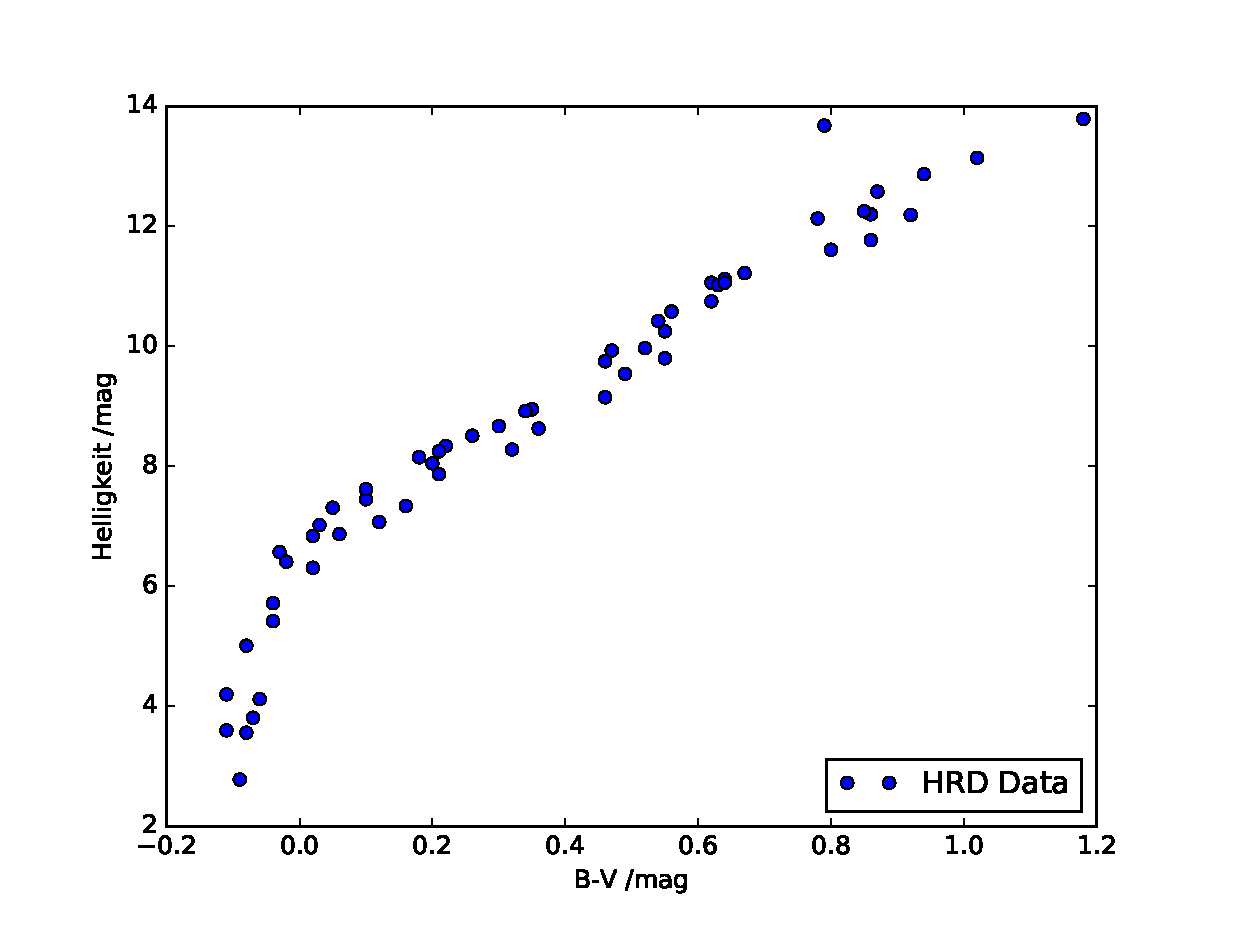
\includegraphics[width=1\textwidth]{hrd_notitle.eps}
	\caption{Scheinbare Helligkeit und Farbindex gegeneinander aufgetragen}
	\label{fig:hrd_unknown}
\end{figure}

Im Diagramm sind die Werte aus Tabelle 4.1 der Anleitung aufgetragen. Die Hauptreihe knickt bei ca. $m=6.6$\,mag und $B-V=0.01$\,mag ab.

\subsection{Aufgabe 2}

Abbildung 4.2 der Anleitung zeigt die abolute Helligkeit aufgetragen gegen den Farbindex, f\"{u}r einige bekannte Sternhaufen. Hier kann man anhand des Farbindexes das ALter des unbekannten Sternhaufens ablesen. Alternativ kann der Farbindex in die effektive Temperatur umgerechnet werden, um Abbildung 4.3 b) verwenden zu k\"{o}nnen. Ohne Information \"{u}ber die Entfernung des Haufens k\"{o}nnen die y-Achsen der Graphen, die jeweils die abolute Helligkeit darstellen, nicht verwendet werden. \\
Die hellsten Sterne sind oft blaue Riesensterne, die eine Farbe zwischen wei"slichem Blau und Blau haben. Das entspricht einem Farbindex von etwa $-0.2$.


\subsection{Aufgabe 3}

Abbildung 4.2 der Anleitung zeigt die abolute Helligkeit aufgetragen gegen den Farbindex, f\"{u}r einige bekannte Sternhaufen. Der Abknickpunkt f\"{u}r $B-V\simeq 0$\,mag steht hier f\'{u}r ein Alter von etwa $4\cdot 10^8$ Jahren (M11).

\subsection{Aufgabe 3}








\section{Hertzsprung-Russell-Diagramme}


\end{document}